\section{Variations without repetition}

A permutation uses all available objects. A variation uses only some of them. The order still matters, but we stop after filling \(k\) positions.

This situation appears when we form a short ordered list from a larger collection: a podium with first, second, and third place; a code made of different symbols; a sequence of selected objects; or an ordered assignment of distinct objects to distinct positions.

\begin{definitionbox}
Let \(A\) be a finite set with \(n\) distinct elements, and let \(k\leq n\). A variation without repetition of length \(k\) is an ordered selection of \(k\) distinct elements from \(A\).
\end{definitionbox}

For example, from
\[
A=\{a,b,c\}
\]
the variations without repetition of length \(2\) are
\[
ab,\quad ac,\quad ba,\quad bc,\quad ca,\quad cb.
\]
The selections \(ab\) and \(ba\) are different, because order matters.

\begin{center}
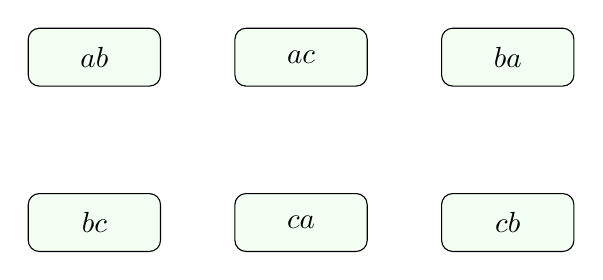
\begin{tikzpicture}[scale=1.05, transform shape]
\foreach \word/\x/\y in {ab/0/2, ac/2.5/2, ba/5/2, bc/0/0, ca/2.5/0, cb/5/0} {
    \node[draw, rounded corners, fill=green!5, minimum width=1.6cm, minimum height=0.7cm] at (\x,\y) {$\word$};
}
\end{tikzpicture}
\end{center}

\begin{theorembox}
The number of variations without repetition of length \(k\) chosen from \(n\) distinct elements is
\[
V(n,k)=n(n-1)(n-2)\cdots(n-k+1)=\frac{n!}{(n-k)!}.
\]
\end{theorembox}

There are \(n\) choices for the first position, \(n-1\) choices for the second position, and so on. Since no element may be repeated, the number of choices decreases after each position is filled. We stop after \(k\) positions, so the product has only \(k\) factors.

A useful mental picture is a row of \(k\) boxes:
\[
\boxed{\phantom{a}}\quad \boxed{\phantom{a}}\quad \cdots \quad \boxed{\phantom{a}}.
\]
The first box has \(n\) possible fillings, the second has \(n-1\), and the process continues until the \(k\)-th box.

\begin{examplebox}
A code consists of three different letters chosen from the six letters
\[
A,B,C,D,E,F.
\]
Order matters and no letter may repeat. The number of possible codes is
\[
V(6,3)=6\cdot5\cdot4=120.
\]
\end{examplebox}

\begin{examplebox}
Eight runners compete for three medals: gold, silver, and bronze. The order matters because the medals are different, and no runner can receive more than one medal. Thus the number of possible medal outcomes is
\[
V(8,3)=8\cdot7\cdot6=336.
\]
\end{examplebox}

\begin{remarkbox}
Use variations without repetition when order matters, only \(k\) positions are filled, and no object may be used more than once. This is the ordered-selection scheme.
\end{remarkbox}
